\section{Performance Evaluation}
\label{Evaluation}

The performance of S-Aligner has been evaluated on the Sunway Taihu
Light supercomputer. We use GRCh38\footnote{available at
  http://hgdownload.cse.ucsc.\\edu/downloads.html} as the human
reference genome.  For the read input data sets we use either
ERR013135\footnote{available at
  ftp://ftp.sra.ebi.ac.uk/vol1/fastq/ERR013/\\ERR013135} or reads
simulated by Mason \cite{mason} or wgsim \cite{wgsim}.\footnote{Note
  that Mason usually generates reads of higher quality but does not
  support long reads.}  We first evaluate the performance in terms of
runtime and mapping accuracy on a single node. Subsequently, we
evaluate the scalability of our implementation by varying the number
of utilized nodes up to 13,312.

\subsection{Single-Node Performance Analysis}

In our single-node experiment, we used the first chromosome of GRCh38 as
reference and 20K reads of length 200 bps generated by Mason as input
data.

First, we evaluated the runtime performance of four different
implementations of edit distance calculation using Myers' algorithm in
one CG: (1) a na\"ive method using the MP only, (2) a na\"ive method
with a nonvectorized SP parallelization, (3) a vectorized Myers
algorithm with the MP only, and (4) our vectorized Myers algorithm
with SP parallelization.

\begin{figure}[!htb]
  \begin{center}
    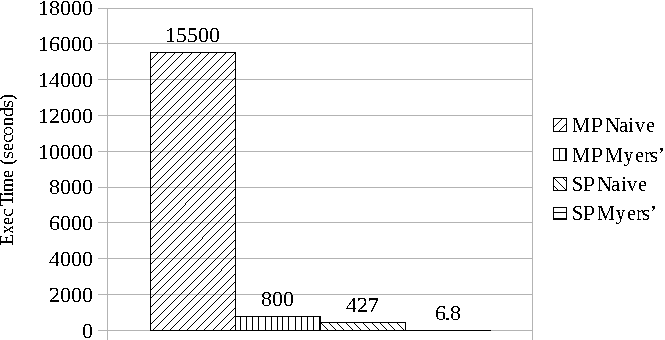
\includegraphics[width=1\linewidth]{figures/VarVerCha}
    \caption{Comparison of the runtimes of four implementations of
      Myers' algorithm on a single CG.}
    \label{VarVerCha}
  \end{center}
\end{figure}

The results in Figure \ref{VarVerCha} show that making
full use of SPs and bit-parallel SIMD vectorization gains dramatic
speedups (118$\times$ and 63$\times$, respectively). Since the MP does
not support high-precision (256-bit integer) extensions, we
implemented a workaround for the high-precision addition
operation. This makes it run slower on a single MP than on a single
SP. Thus, using SPs can gain a superlinear speedup in this
application. Furthermore, our bit-parallel SIMD implementation is able
to update 256 cells simultaneously using 23 instructions (i.e., 0.09
instructions per cell) while the na\"ive implementation computes one
cell using 6 instructions. This results in a theoretical speedup of
$\sim$67$\times$, which explains the actually achieved speedup of
63$\times$.

Second, we evaluated the impact of using asynchronous filtration and
the impact of using DMA intrinsics versus \texttt{memcpy}. The results
are shown in Figure \ref{VarOptCha}.

\begin{figure}[!htb]
  \begin{center}
    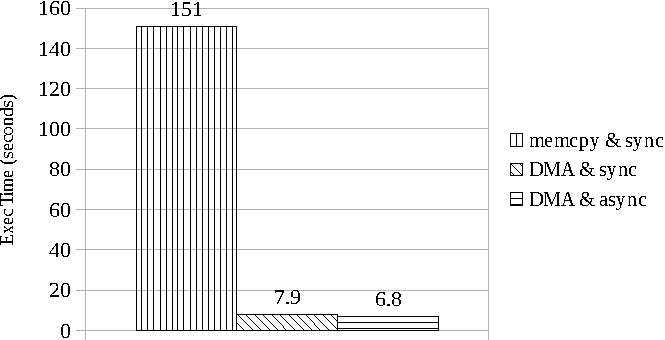
\includegraphics[width=1\linewidth]{figures/VarOptCha}
    \caption{Evaluation with and without I/O optimizations.}
    \label{VarOptCha}
  \end{center}
\end{figure}

The results demonstrate that DMA fetching is key for achieving high
performance when using SPs, since a speedup of $\sim$22$\times$ is
gained over \texttt{memcpy}. This can be attributed to two factors:
(1) DMA transfers require fewer compute resources since they are
performed by the memory controller, whereas \texttt{memcpy} uses an SP
to write data to memory; and (2) DMA fetching can be performed
asynchronously, thus enabling the latency of fetching data to be
hidden by computation. Furthermore, asynchronous filtration gains
$\sim$15\% speedup.

In summary, the architecture of SW26010 differs significantly from a
conventional x86\_64 CPU. Straightforward migration of code therefore
typically results in an inefficient implementation on SW26010, and
architecture-specific optimizations are required in order to achieve
high performance. As a case study, we compiled and executed
multithreaded BWA \cite{bwa} (one of the most well-known {\em any-best
  mappers}) on SW26010. It runs two times slower than S-Aligner, while
finding significantly fewer locations, showing the importance of
making changes according to this specific architecture.

\subsection{Comparison with RazerS3}

In our experiment with RazerS3, we used the first chromosome from GRCh38 as
reference and various numbers of reads from ERR013135. The runtime of
S-Aligner on a single SW26010 node was compared with that of RazerS3, a
representative all-mapper. Since RazerS3 does not support ShenWei's
architecture, we ran it on a machine with Intel processors using
multithreading with default parameters (e.g., the accuracy parameter
is set to 98\%). Measured runtimes are shown in Table
\ref{SingleNode}.  One can see that S-Aligner executed on a single
SW26010 (260 cores running at 1.45 GHz) outperforms RazerS3 running on
eight Xeon E7-8860v3 CPUs (128 cores running at 3.2 GHz).

\begin{table}
  \begin{threeparttable}
    \caption{Runtime comparison between S-Aligner running on a single
      CG and RazerS3 running on a single node with eight Xeon
      E7-8860v3 CPUs.}
    \label{SingleNode}
    \begin{tabular}{@{\extracolsep{2pt}}rrrrr}
      \hline
      \multicolumn{1}{c}{Ref} &
      \multicolumn{2}{c}{Reads} &
      \multicolumn{2}{c}{Time(s)}\\
      \cline{2-3}
      \cline{4-5}
      \multicolumn{1}{c}{\#bps} &
      \multicolumn{1}{c}{Count} &
      \multicolumn{1}{c}{\#bps} &
      \multicolumn{1}{c}{RazerS3\tnote{\textdagger}} &
      \multicolumn{1}{c}{S-Aligner\tnote{\textdaggerdbl}}\\
      \hline
      116M & 40M & 108 &  939 & 405\\
      253M & 40M & 108 &  3,044 & 892\\
      253M & 40M & 200 &  3,430 & 2,580\\
      \hline
    \end{tabular}
    \begin{tablenotes}
    \item[\textdagger] Result is from a machine with eight Xeon
      E7-8860v3 (128 cores up to 3.20 GHz).
    \item[\textdaggerdbl] Result is from a node with a SW26010 (260
      cores with frequency of 1.45 GHz).
    \end{tablenotes}
  \end{threeparttable}
\end{table}

Rabema \cite{rabema} (Read Alignment BEnchMark) is a well-defined read
alignment benchmark that can evaluate the quality of read mappers in
both {\em all} and {\em any-best} mode. We evaluated the accuracy of
S-Aligner in {\em all} mode based on Rabema by using the result of RazerS3
with the accuracy parameter set to 100\% as gold standard. S-Aligner
can find up to 99.8\% of the normalized intervals found by RazerS3
(100\% accuracy), which is higher than the accuracy of RazerS3
executed with default parameters (98\% accuracy). Detailed results are
provided in Table~\ref{AccuEval}.

\begin{table}
  \begin{threeparttable}
    \caption{Accuracy evaluation of S-Aligner for both real and
      simulated data.}
    \label{AccuEval}
    \begin{tabular}{@{\extracolsep{2pt}}rrrrrr}
      \hline
      \multicolumn{1}{c}{Chrom} &
      \multicolumn{3}{c}{Reads} &
      \multicolumn{1}{c}{\multirow{2}{*}{Interv. found}} \\
      \cline{2-4}
      \multicolumn{1}{c}{Index} &
      \multicolumn{1}{c}{Origin} &
      \multicolumn{1}{c}{Count} &
      \multicolumn{1}{c}{\#bps} \\		
      \hline
      1\textsuperscript{st} & ERR013135 & 20,000 & 108 & 99.34\%\\
      1\textsuperscript{st} & Mason &  20,000 & 200 & 99.82\%\\
      \hline
    \end{tabular}
  \end{threeparttable}
\end{table}

\subsection{Scalability Analysis}

To evaluate weak and strong scalability, we measured the runtimes of
S-Aligner using different numbers of nodes ranging from 13 to
13,312. The full GRCh38 assembly of the human genome was used as
reference. Input reads were simulated by Mason with an error rate of
4\% and a length of 200 bps. Weak scalability was measured for numbers
of nodes ranging from 13 to 3,328 by increasing the number of input
reads from 16 million to 4 billion, correspondingly. Strong
scalability was measured by increasing the number of nodes from 3,328
to 13,312 while keeping the number of input reads constant at 4
billion. We measured the performance in terms of {\em read base-pairs
  processed per second} in total and normalized per node (see
Table \ref{paraexp}). Figure \ref{VarProcCha} shows the achieved
speedups and efficiencies. The results demonstrate weak scalability
since the normalized node performance is almost constant for the
number of nodes ranging from 13 to 3,328. Furthermore, the node
performance only slightly decreases when increasing the number of
nodes from 3,328 to 13,312 while keeping the number of input reads
constant at 4 billion, thus demonstrating strong scalability for
sufficiently large input datasets.

\begin{table}[!htb]
  \begin{threeparttable}
    \caption{Performance and runtime evaluation of S-Aligner using
      different numbers of nodes.}
    \label{paraexp}
    \begin{tabular}{rrrrrr}
      \hline
      \multicolumn{1}{c}{\multirow{2}{*}{\# Nodes}} &
      \multicolumn{2}{c}{Reads}  &
      \multicolumn{1}{c}{\multirow{2}{*}{Time(s)}} &
      \multicolumn{2}{c}{Performance (bpps)} \\
      \cline{2-3}
      \cline{5-6}
      \multicolumn{1}{c}{} &
      \multicolumn{1}{c}{Count} &
      \multicolumn{1}{c}{\# bps} & &
      \multicolumn{1}{c}{Total (M)} &
      \multicolumn{1}{c}{Node (K)}\\
      \hline
      13 & 16M & 200 & 1,315 & 2.43 & 185.43\\
      52 & 64M & 200 & 1,321 & 9.69 & 184.80\\
      208 & 256M & 200 & 1,321 & 38.76 & 184.66\\
      832 & 1,024M & 200 & 1,327 & 154.33 & 184.59\\
      3,328 & 4,096M & 200 & 1,349 & 607.26 & 179.67\\
      13,312 & 4,096M & 200 & 344 & 2,381.40 & 178.90\\
      \hline
    \end{tabular}
    \begin{tablenotes}
    \item
      \# Nodes is the number of nodes involved in computing..
    \item
      bpps is short for million base pairs processed per second.
    \item
      M (K) indicates that column is presented in millions (thousands).
    \end{tablenotes}
  \end{threeparttable}
\end{table}

\begin{figure}[!htb]
  \begin{center}
    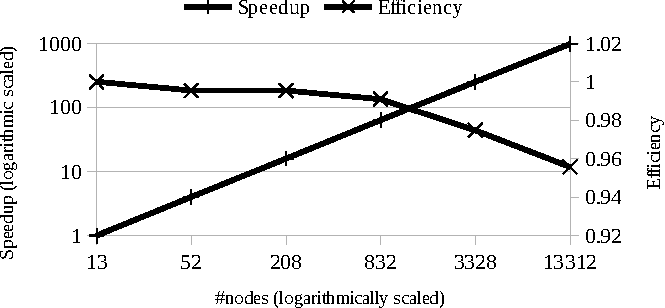
\includegraphics[width=1\linewidth]{figures/VarProcCha}
    \caption{Speedup and efficiency of S-Aligner for different numbers
      of nodes.}
    \label{VarProcCha}
  \end{center}
\end{figure}
